% !TeX spellcheck = en_US
% Chapter 1

%\chapter{Chapter Title Here} % Main chapter title
%
%\label{Chapter1} % For referencing the chapter elsewhere, use \ref{Chapter1} 

%----------------------------------------------------------------------------------------

% Define some commands to keep the formatting separated from the content 

%\newcommand{\option}[1]{\texttt{\itshape#1}}

%----------------------------------------------------------------------------------------

\chapter{Methodology}\label{ch: methodology}
	The host galaxy of the black hole is modeled as two mass distributions that are superimposed, one for dark matter and the other one for all the luminous or baryonic matter.
	\begin{figure}[h]
		\centering
		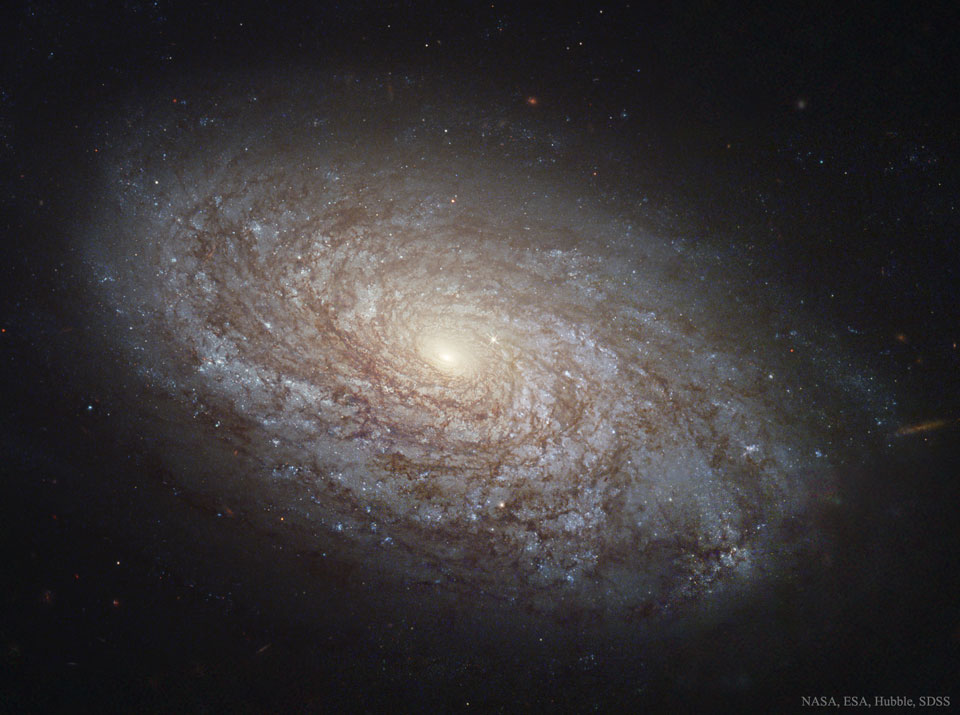
\includegraphics[width=0.8\linewidth]{Figures/NGC4414_modified}
		\caption{NGC4414 galaxy as seen by the Hubble telescope.}
	\end{figure}
	
	The dark matter halo used follows a NFW (Navarro–Frenk–White) profile, baryonic matter is divided in stars and gas. For the gas a power law profile with $r^{-2.2}$ is used, while for stars a Hernquist model is applied \cite{tanaka2009assembly, choksi2017recoiling}. The sum of all these components accounts for the total mass of the host ($M_\text{total}$), which remains constant through a simulation. The amount of baryonic matter is given by the baryonic fraction parameter ($f_b$), and the mass of stars by the stellar fraction parameter ($f_s$). Cumulative masses at the virial radius are defined as follows (Appendix A \autoref{sec: cd_vr}):
	\begin{equation}
		M_\text{DM}(R_\text{vir}) = (1 - f_b)M_\text{total}
	\end{equation}
	\begin{equation}
		M_\text{stars}(R_\text{vir}) = f_sf_bM_\text{total}
	\end{equation}
	\begin{equation}
		M_\text{gas}(R_\text{vir}) = (1 - f_s)f_bM_\text{total}
	\end{equation}
	
	Some of the simulation parameters are dependent of the cosmological model used, unless otherwise specified, all data is acquired using the $\Lambda$-CDM model with a matter density parameter $\Omega_M = 0.309$, $\Omega_\Lambda = 0.6911$, and a baryonic fraction $f_b = 0.156$ \cite{choksi2017recoiling}. Also, as \citeauthor{binney2011galactic}, argue, about 1 \% of the stellar mass of galaxies, such as The Milky Way, are contained in the stellar halo, $f_s \equiv 0.01$, unless otherwise stated.
	
	\section{Densities profiles}
		\subsection{Dark matter halo}
			For a dark matter halo following a NFW profile, the density at some distance $r$ is given by the formula:
			\begin{equation}\label{eq: dmdensity}
				\rho_\text{DM}(r) = \dfrac{\rho_0^\text{DM}}{\frac{r}{R_s}\left(1 + \frac{r}{R_s}\right)^2}
			\end{equation}
			
			Where $R_s$ and $\rho_0^\text{DM}$ are constants for a given dark matter halo. For a triaxial potential, it is said that density is constant within ellipsoids of ellipsoidal radius $m$. Using the Cartesian coordinates $x_1$, $x_2$, $x_3$ and $a_1$, $a_2$, $a_3$ the semi-axis of the ellipsoid, $m$ is defined as follows:
			\begin{equation}
				m^2(\vec{x}) \equiv a_1^2\left[\left(\dfrac{x_1}{a_1}\right)^2 + \left(\dfrac{x_2}{a_2}\right)^2 + \left(\dfrac{x_3}{a_3}\right)^2\right] = x_1^2 + \left(\dfrac{a_1}{a_2}\right)^2x_2^2 + \left(\dfrac{a_1}{a_3}\right)^2x_3^2
			\end{equation}
			
			Considering a concentration parameter $c(M_\text{total}, z)$ of dark matter in the halo, the following relation holds for the viral radius $R_\text{vir}$ and the scale radius $R_s$:
			\begin{equation}\label{eq: virialConcentration}
				R_\text{vir} = c(M_\text{total}, z)R_s
			\end{equation}
			
			Where the concentration parameter, dependence with the dark matter halo mass ($M_\text{total}$) and redshift is given by: 
			\begin{equation}
			c(M_\text{total}, z) = c_0(z)\left(\dfrac{M_\text{total}}{10^{13}M_\theta}\right)^{\alpha(z)}
			\end{equation}
			
			where $\alpha(z)$ and $c_0(z)$ were fitted using simulation data to the following functions \cite{choksi2017recoiling}:
			\begin{equation}
				c_0(z) = \dfrac{4.58}{2}\left[\left(\dfrac{1 + z}{2.24}\right)^{0.107} + \left(\dfrac{1 + z}{2.24}\right)^{-1.29}\right]
			\end{equation}
			
			\begin{equation}
				\alpha(z) = -0.0965 \exp\left(-\dfrac{z}{4.06}\right)
			\end{equation}
			
			\begin{figure}[h]
				\centering
				\includegraphics[width=0.7\linewidth]{"../Files/Week 3/darkmatter_concentration"}
				\caption{Dark matter concentration parameter as a function of the halo mass and the redshift.}
				\label{fig: dmconcentration}
			\end{figure}
			
			For a fixed halo mass, as time passes (smaller redshift), concentration of dark matter will increase, as can be shown on \autoref{fig: dmconcentration}, nevertheless for high redshifts concentration is approximately constant at $c \approx 3$ for all halos \cite{choksi2017recoiling}. Thus, the dark matter concentration parameter for all the simulations is fixed at this value.
	
		\subsection{Stellar density}
			Stellar density is modeled as a Hernquist profile with half-mass radius $R_{1/2} = 0.01 R_\text{vir}$, as in \citeauthor{choksi2017recoiling}. Density for a Hernquist profile is given by \cite{hernquist1990analytical}:
			\begin{equation}\label{eq: sdensity}
				\rho_s(r) = \dfrac{f_sf_bM_\text{total} \mathcal{R}_s}{2\pi r(r + \mathcal{R}_s)^3} \qquad \text{$\mathcal{R}_s$ is known as scale length}
			\end{equation}
			
			The half-mass radius, as the name implies, is the distance at which the cumulative mass is half the total mass \cite{hernquist1990analytical}. By using the result in \autoref{eq: r_vir}:
			\begin{equation}
				R_{1/2} = \left(1 + \sqrt{2}\right)\mathcal{R}_s = 0.01\left({\dfrac{M_\text{total}G}{100 H(t)^2}}\right)^{1/3}
			\end{equation}
			
			From which the scale length can be set as a function of the time when the kick occurs, and the mass of the host, as:
			\begin{equation}
				\mathcal{R}_s = \dfrac{0.01}{\left(1 + \sqrt{2}\right)}\left({\dfrac{M_\text{total}G}{100 H(t)^2}}\right)^{1/3} \approx 6.835\times 10^{-4}\left({\dfrac{M_\text{total}}{H(t)^2}}\right)^{1/3}
			\end{equation}
		\subsection{Gas density}
			For high redshift the baryonic profile resembles that of a gaseous galaxy, \citeauthor{choksi2017recoiling} use a constant density gas core of $r_0 = 1$ pc, followed by a power law of $r^{-n} = r^{-2.2}$. Density is described as follows: for $r \gg r_0$, $\rho_\text{gas}(r)\propto r^{-n}$ while for $r \ll r_0$, $\rho_\text{gas}(r) \approx \rho_0^\text{gas}$.
			\begin{equation}\label{eq: rdensity}
				\rho_\text{gas}(r) = \dfrac{\rho_0^\text{gas}}{\left(1 + \dfrac{r}{r_0}\right)^n}
			\end{equation}
	
	\section{Equation of motion}
		Trajectories of the kicked black holes are obtained by numerically solving the equation of motion on \autoref{eq: equationMotion}, where the first term on the right side of the equation is acceleration due to gravity, the second accounts for the drag of dynamical friction, while the third is the deaceleration due to mass accretion of the black hole \cite{tanaka2009assembly, choksi2017recoiling}.
		\begin{equation}\label{eq: equationMotion}
			\ddot{\vec{x}}(\vec{x}, \dot{\vec{x}}) = a_\text{grav}(\vec{x})\hat{x} + \left(a_\text{DF}(\vec{x}, \dot{\vec{x}})-\dot{x}\dfrac{\dot{M_\bullet}(x, \dot{x})}{M_\bullet}\right)\dot{\hat{x}} \qquad \text{where $M_\bullet$ is the black hole mass}
		\end{equation}
		
		\subsection{Dynamical friction}
			As the black hole travels through the galaxy, dark matter, stars and gaseous materials from the medium interact with the black hole adding a drag force due to friction. Drag force is different in nature depending on its source, collisionless components, such as dark matter and stars, apply a drag force to the black hole that follows the standard Chandrasekhar formula \cite{binney2011galactic, madau2004effect, tanaka2009assembly, choksi2017recoiling}.
			\begin{equation}\label{eq: df_cl}
				a_\text{DF}^\text{cl}(\vec{x}, \dot{\vec{x}}) = -\dfrac{4\pi G^2}{\dot{x}^2} M_\bullet\rho(\vec{x})\ln\Lambda\left(\erf{X} - \dfrac{2}{\sqrt{\pi}}Xe^{-X^2}\right)\text{, } \quad \rho(\vec{x}) = \rho_\text{DM}(\vec{x}) + \rho_\text{stars}(\vec{x})
			\end{equation}
			\begin{equation}
				X \equiv \dfrac{|\dot{x}|}{\sqrt{2}\sigma_\text{DM}} \qquad \text{with } \sigma_\text{DM} = \sqrt{\dfrac{GM_\text{DM}}{2R_\text{vir}}}
			\end{equation}
			
			$\sigma_\text{DM}$ is called the local velocity dispersion of the dark matter halo, and since varies little over the entire host, can be taken as constant \cite{tanaka2009assembly, choksi2017recoiling}. The Coulomb logarithm ($\ln\Lambda$) is not known but authors take it in the range of 2 - 4 \cite{choksi2017recoiling}. Gas on the other hand is collisional, special care must be taken since gas can cool behind a passing object, such as a black hole \cite{choksi2017recoiling}. A hybrid model for the drag force was proposed by \citeauthor{tanaka2009assembly}, in which both subsonic and supersonic velocities are possible. To do so, a mach number was defined as:
			\begin{equation}
				\mathcal{M}(\dot{x}) \equiv \dfrac{|\dot{x}|}{c_s}
			\end{equation}
			
			where $c_s$ is the local sound speed, which depends on local temperature. It was found that temperature inside the halo varies less than a factor of 3, thus on the simulation it is assumed that the entire halo is isothermal at the virial temperature ($T_\text{vir}$) \cite{choksi2017recoiling}. The isothermal sound speed is \cite{barkana2001beginning}:
			\begin{equation}\label{eq: soundSpeed}
				c_s = \sqrt{\dfrac{\gamma R}{\mathcal{M}_w}T_\text{vir}} = \sqrt{\dfrac{\gamma R}{\mathcal{M}_w}\left(\dfrac{\mu m_p G M_\text{total}}{2k_BR_\text{vir}}\right)} = \sqrt{\dfrac{\gamma R\mu m_pG}{2\mathcal{M}_wk_B}} \sqrt{\dfrac{M_\text{total}}{R_\text{vir}}} \approx 0.614 \sqrt{\dfrac{M_\text{total}}{R_\text{vir}}}\text{ kpcGyr$^{-1}$}
			\end{equation}
			
			where $\mu$ is the value of the mean molecular weight of the gas ($\mathcal{M}_w$), $m_p$ is the proton mass and $\gamma$ is the adiabatic index \cite{barkana2001beginning}. Approximating the gas to a monoatomic one $\gamma \approx 5/3$, yields the last expression on \autoref{eq: soundSpeed}. By knowing $\mathcal{M}$, the acceleration caused by gas can be written as \cite{tanaka2009assembly, choksi2017recoiling}:
			\begin{equation}\label{eq: df_c}
				a^\text{c}_\text{DF}(\vec{x}, \dot{\vec{x}}) = -\dfrac{4\pi G^2}{\dot{x}^2}M_\bullet\rho_\text{gas}(\vec{x})f(\mathcal{M})
			\end{equation}
			
			with
			\begin{equation}
				f(\mathcal{M}) = \left\{
				\begin{matrix}
				0.5\ln\Lambda \left[\erf{\dfrac{\mathcal{M}}{\sqrt{2}}} - \sqrt{\dfrac{2}{\pi}}\mathcal{M}e^{-\mathcal{M}^2/2}\right]& \text{if $\mathcal{M} \leq 0.8$}\\
				1.5\ln\Lambda \left[\erf{\dfrac{\mathcal{M}}{\sqrt{2}}} - \sqrt{\dfrac{2}{\pi}}\mathcal{M}e^{-\mathcal{M}^2/2}\right] & \text{if $0.8 < \mathcal{M} \leq \mathcal{M}_{eq}$}\\
				0.5\ln\left(1 - \mathcal{M}^{-2}\right) + \ln\Lambda & \text{if $\mathcal{M} > \mathcal{M}_{eq}$}
				\end{matrix}
				\right.
			\end{equation}
			
			$M_{eq}$ is the mach number that fulfills the following equation:
			\begin{equation}\label{eq: machEq}
				\ln\Lambda\left[1.5\left(\erf{\dfrac{\mathcal{M}}{\sqrt{2}}} - \sqrt{\dfrac{2}{\pi}}\mathcal{M}e^{-\mathcal{M}^2/2}\right) - 1\right] - 0.5\ln\left(1 - \mathcal{M}^{-2}\right) = 0
			\end{equation}
			
			Numerically solving \autoref{eq: machEq}, yields $M_{eq} \approx 1.731$ for a value of the Coulomb logarithm $\ln\Lambda = 2.3$. The full acceleration due to dynamical friction is given by the sum of the noncollisional drag on \autoref{eq: df_cl} and \autoref{eq: df_c}:
			\begin{equation}
				a_\text{DF}(\vec{x}, \dot{\vec{x}}) = a_\text{DF}^\text{cl}(\vec{x}, \dot{\vec{x}}) + a_\text{DF}^\text{c}(\vec{x}, \dot{\vec{x}})
			\end{equation}
		
		\subsection{Accretion onto the black hole}
			As the black hole accretes matter from the surroundings, an acceleration appears, due to the second law of Newton:
			\begin{equation}
				\vec{F} = \dfrac{d\vec{P}}{dt} = \dot{\vec{x}}\dot{M}_\bullet + M_\bullet\ddot{\vec{x}}
			\end{equation}
			
			By considering conservation of momentum:
			\begin{equation}
				\ddot{\vec{x}} = - \dot{\vec{x}}\dfrac{\dot{M}_\bullet}{M_\bullet}
			\end{equation}
			
			Two schemes describe the speed at which the black hole gains mass, on the first one the black hole undergoes Bondi-Hoyle-Littleton accretion \cite{tanaka2009assembly, choksi2017recoiling}:
			\begin{equation}
				\dot{M}_\bullet^\text{BHL}(\vec{x}, \dot{\vec{x}}) = \dfrac{4\pi G^2 \rho_G(\vec{x})M^2_\bullet}{\left(c_s^2 + \dot{x}^2\right)^{3/2}} \qquad \text{with } \rho_B(\vec{x}) = \rho_\text{stars}(\vec{x}) + \rho_\text{gas}(\vec{x})
			\end{equation}
			
			But, there is a limit of accretion for the black hole given by the Eddington luminosity:
			\begin{equation}\label{eq: eddington}
				\dot{M}_\bullet^\text{Edd} = \dfrac{(1 - \epsilon)M_\bullet}{\epsilon t_\text{Edd}} \qquad \epsilon = 0.1, \quad t_\text{Edd} = 0.44 \text{ Gyr}
			\end{equation}
			
			Thus, the final accretion rate is given by:
			\begin{equation}
				\dot{M}_\bullet(\vec{x}, \dot{\vec{x}}) = \left\{
				\begin{array}{lc}
				\dot{M}_\bullet^\text{BHL}(\vec{x}, \dot{\vec{x}}) & \text{if $\dot{M}_\bullet^\text{BHL} < \dot{M}_\bullet^\text{Edd}$} \\
				\dot{M}_\bullet^\text{Edd} & \text{else}
				\end{array}
				\right.
			\end{equation}
	
	\subsection{Initial conditions and numerical integration}
		For all simulations the virial radius remains constant through the simulation. The virial radius is fixed at the start of every simulation depending on the redshift at which the kick occurs, the chosen densities profiles and the mass of the host galaxy. Sound speed also remains constant for a simulation, as it depends on $R_\text{vir}$ and the mass of the host. Cosmological acceleration is ignored at all times as in \citeauthor{tanaka2009assembly}, as it has been found that it only marginally affects black hole orbits \cite{choksi2017recoiling}. The initial position of the black hole is always $\vec{x} = (1, 1, 1)$ pc.
		
		Numerical integration is carried out using a Leapfrog scheme on REBOUND with the C programming language \cite{larson2017modeling}, with time steps of a thousand years, the simulations are stopped when the system destabilizes and starts gaining energy, due to singularities at $x \rightarrow 0$ and $\dot{x} \rightarrow 0$, or if they simply last more than the current age of the universe. 
		
	\section{Definitions}
%		\subsection{Escape velocity}
%			Minimum initial velocity required for the maximum distance of a single orbit of the black hole to stay outside $0.01R_\text{vir}$ by $z = 0$, $z = 6$ or 10 \% of the age of the universe at the moment of the kick \cite{tanaka2009assembly, choksi2017recoiling}.
		
		\subsection{Return time}
			Time required by the black holes orbit to have a maximum distance of less than $0.01R_\text{vir}$.
			
		\subsection{Return mass}
			Mass at the return time of the black hole.
			
	\section{Spherical setup}
	\subsection{Virial radius}
		Since all of the density profiles are spherically symmetrical, it follows from \autoref{eq: R_vir_def} that:  
		\begin{equation}
		\dfrac{M_\text{total}}{4/3\pi R_\text{vir}^3} = 75\dfrac{H(t)^2}{\pi G}
		\end{equation}
		\begin{equation}\label{eq: r_vir}
		R_\text{vir} = \left({\dfrac{M_\text{total}G}{100 H(t)^2}}\right)^{1/3}
		\end{equation}
	
	\subsection{Dark matter halo}
		For a dark matter halo following a NFW profile, the cumulative mass $M_\text{DM}(r)$ within some radius $r$ is given by the integral of the density over a volume. Since \autoref{eq: dmdensity} is spherically symmetrical, the only dependance of the integral is with distance. On \autoref{eq: cumulativeDM} the $r'^2$ comes from the Jacobian of spherical coordinates, and the $4\pi$ from the solid angle.
		\begin{equation}\label{eq: cumulativeDM}
			M_{DM}(r) = \int\limits_0^{r} 4\pi {r'}^2\rho_\text{DM}(r')dr' = 4\pi\rho_0^\text{DM}R_s^3\left[\ln\left(\dfrac{R_s + r}{R_s}\right) - \dfrac{r}{R_s + r}\right]
		\end{equation}
		
		By using \autoref{eq: virialConcentration} one can obtain the value of $\rho_0^\text{DM}$ by evaluating \autoref{eq: cumulativeDM} at $R_\text{vir}$.
		\begin{equation}\label{eq: dmM_virial}
		M_\text{DM}(R_\text{vir}) = 4\pi\rho_0^\text{DM}R_s^3 \left[\ln\left(\dfrac{R_s + c(M_\text{total}, z)R_s}{R_s}\right) - \dfrac{c(M_\text{total}, z)R_s}{R_s + c(M_\text{total}, z)R_s}\right] = (1 - f_b)M_\text{total}
		\end{equation}
		\begin{equation}\label{eq: rho0dm}
		\rho_0^\text{DM} = \dfrac{(1 - f_b)M_\text{total}}{4\pi \left(\dfrac{R_\text{vir}}{c(M_\text{total}, z)}\right)^3 \left[\ln\left(1 + c(M_\text{total}, z)\right) - \dfrac{c(M_\text{total}, z)}{1 + c(M_\text{total}, z)}\right]}
		\end{equation}
	
	\subsection{Stellar profile}		
		Integrating \autoref{eq: sdensity} from $0$ to $r$ yields:
		\begin{equation}
			M_s(r) = \dfrac{f_sf_bM_\text{total} r^2}{(r + \mathcal{R}_s)^2}
		\end{equation}
	
	\subsection{Gas profile}		
		The cumulative mass is found by integrating \autoref{eq: rdensity} in spherical coordinates.
		\begin{equation}
			\begin{array}{rl}
			M_\text{gas}(r) 
			& = 4\pi\rho_0^\text{gas} r_0^3\int\limits_{0}^{u}\dfrac{u'^2}{(1 + u')^n}du' \\
			& = 4\pi\rho_0^\text{gas} r_0^3\left(u + 1\right)^{-n}\dfrac{-(u + 1)(nu)^2 + 2[(u + 1)^n - u^3-1] + nu[3u^2 + u - 2]}{(n - 3)(n - 2)(n - 1)}
			\\
			& \text{where $u = r/r_0$, for $u \leq 0$ and $n \neq {1, 2, 3}$}
			\end{array}
		\end{equation}
		
		The value of the constant $\rho_0^\text{gas}$ is found using a similar process as in \autoref{eq: dmM_virial} and \ref{eq: rho0dm}.
		\begin{equation}
			\rho_0^\text{gas} = \dfrac{(1 - f_s) f_bM_\text{total}}{(M_\text{gas}(R_\text{vir}) / \rho_0^\text{gas})}
		\end{equation}
		
		All of the profiles are shown on \autoref{fig: massprofiles}, where the effect of the stellar fraction can be seen.
		
		\begin{figure}[h]
			\centering
			\begin{subfigure}[b]{0.49\textwidth}
				\includegraphics[width=\textwidth]{"../Files/Week 6/density_mass_fs01"}
				\caption{Stellar fraction $f_s = 0.01$.}
				\label{fig: baryonicprofilehigh}
			\end{subfigure}
			~ 
			\begin{subfigure}[b]{0.49\textwidth}
				\includegraphics[width=\textwidth]{"../Files/Week 6/density_mass_fs3"}
				\caption{Stellar fraction $f_s = 0.30$.}
				\label{fig: baryonicprofilelow}
			\end{subfigure}
			\caption{Mass distributions for $R_\text{vir} = 0.69$ kpc (red line), $c = 4$, and $f_b = 0.156$.}
			\label{fig: massprofiles}
		\end{figure}
	
	\section{Triaxial setup}
		\begin{figure}[h]
			\centering
			\begin{subfigure}[t]{0.49\textwidth}
				\includegraphics[width = \textwidth]{"../Files/Week 7/symmetric"}
				\caption{Spherical case}
				\label{fig: symmetricDensity3d}
			\end{subfigure}
			~ 
			\begin{subfigure}[t]{0.49\textwidth}
				\includegraphics[width=\textwidth]{"../Files/Week 7/triaxial"}
				\caption{Triaxial case with ($a_1$:$a_2$:$a_3$) = (1:0.5:0.3)}
				\label{fig: triaxialDensity3d}
			\end{subfigure}
			\begin{subfigure}[t]{0.6\textwidth}
				\includegraphics[width=\textwidth]{"../Files/Week 7/ellipsoid_"}
				\caption{Equicentred ellipsoids with ($a_1$:$a_2$:$a_3$) = (1:0.5:0.3)}
			\end{subfigure}
			\caption{Dark matter densities comparison between spherical and triaxial cases.}
			\label{fig: symmetricTriaxial}
		\end{figure}
	
		The host galaxy is modeled as a dark matter halo, stars and gas, just as the spherical case. Much of the profiles for each of the components remains the same, the only difference is that a thin shell of uniform density will have the geometry of an ellipsoid, and not that of a sphere. This is achieved by defining an ellipsoid radius $m$, that can be replaced for the spherical radius $r$, on equations \ref{eq: dmdensity}, \ref{eq: sdensity} and \autoref{eq: rdensity}, as can be seen on \autoref{fig: symmetricTriaxial}. 
		
		A thin shell, whose inner and outer skins are the surfaces $m$ and $m + \delta m$ is described by \autoref{eq: m2}, where $\tau \geq 0$ labels the surfaces \cite{binney2011galactic}.
		\begin{equation}\label{eq: m2}
		m^2(\vec{x}, \tau) = a_1^2\left(\frac{x_1^{2}}{\tau + a_{1}^{2}} + \frac{x_2^{2}}{\tau + a_{2}^{2}} + \frac{x_3^{2}}{\tau + a_{3}^{2}}\right)
		\end{equation}
		
		Densities are used for the calculation of the dynamical friction and accretion onto the black hole. Although one might think that by integrating the density over an elliptical volume, the acceleration due to gravity would be given by $a_\text{grav} = GM(m)/m^2$, the later is not true because two points $(x_1, x_2, x_3)$ and $(x_1', x_2', x_3')$ might have the same cumulative mass at $m$ (black line), but the effective gravitational mass acting at each point is completely different (blue and orange lines) as it is shown in \autoref{fig: triaxial_mass_issue}.
		\begin{figure}[h]
			\centering
			\includegraphics[width = 0.4\linewidth]{"../Files/Week 7/triaxial_mass_issue"}
			\caption{Although the cumulative mass at the orange and blue dots is the same, the effective gravitational mass is different.}
			\label{fig: triaxial_mass_issue}
		\end{figure}
	
		Because of this, the potential due to a given triaxial density must be found. Calculating the gravitational potential for such configuration, challenged some great minds of the XVIII and XIX centuries \cite{binney2011galactic}. To do so, the contributions of all ellipsoidal shells that make up the profile are taken into account, following \citeauthor{binney2011galactic}:
		\begin{equation}
			\psi(m) \equiv \int\limits_{0}^{m^2} \rho(m'^2)dm'^2 = \int\limits_{0}^{m} 2m'\rho(m')dm' 
		\end{equation}
		
		The potential of any body in which $\rho = \rho(m^2)$ is \cite{binney2011galactic}:
		\begin{equation}\label{eq: generalPotential}
		\Phi(\vec{x}) = -\pi G \dfrac{a_2a_3}{a_1}\int\limits_{0}^{\infty}\dfrac{\psi(\infty) - \psi(m)}{\sqrt{(\tau + a_1^2)(\tau + a_2^2)(\tau + a_3^2)}}d\tau \qquad m = m(\vec{x}, \tau)
		\end{equation}
		\begin{table}[h]
			\centering
			\caption{$\psi$ values for the studied density profiles}
			\begin{tabular}{c|c}
				\hline
				\textbf{Profile} & $\psi(\infty) - \psi(m)$ \\
				\hline
				\rule{0pt}{4ex} 
				\textbf{NFW} & $\dfrac{2R_s^3\rho_0^\text{DM}}{R_s + m(\vec{x}, \tau)}$\\
				%				\hline
				\textbf{Hernquist} & $\dfrac{M_s\mathcal{R}_s}{2\pi\left(\mathcal{R}_s + m(\vec{x}, \tau)\right)^2}$ \\
				%				\hline
				\textbf{Power-law} & $\dfrac{2 \rho_0^\text{gas} \left(\frac{m(\vec{x}, \tau) + r_{0}}{r_{0}}\right)^{- n} \left(m(\vec{x}, \tau) + r_{0}\right) \left(m(\vec{x}, \tau) \left(n - 1\right) + r_{0}\right)}{\left(n - 2\right) \left(n - 1\right)}$
				\\
				\hline
			\end{tabular}
		\end{table}
		
		Most of the triaxials potentials cannot be analytically integrated, nevertheless it can be done numerically. Since the gravitational acceleration is given by the gradient of the potential, to numerically calculate the gradient, a total of 6 numerical integrals must be done (two for each dimension, and then numerically differentiate). Another option is to take advantage of the fact that $\vec{x}$ and $\tau$ are independent variables, thus:
		\begin{equation}
			\nabla \int f(\vec{x}, \tau)d\tau = \int [\nabla f(\vec{x}, \tau)] d\tau
		\end{equation}
		
		By doing this, the number of numerical integrals reduces to 3. Defining a vector $\vec{\phi}$, whose components are given by:
		\begin{equation}
			\phi_i(x_i, \tau) = \dfrac{x_i}{\left(\tau + a_i^2\right)^{\frac{3}{2}} \prod\limits_{i \neq j}^3\sqrt{\tau + a_j^2}}, \qquad \vec{\phi}(\vec{x}, \tau) = (\phi_1(x_1, \tau), \phi_2(x_2, \tau), \phi_3(x_3, \tau))
		\end{equation}
		
		Potentials for each of the components of the galaxy are found by calculating $\psi(\infty) - \psi(m)$ and replacing on \autoref{eq: generalPotential}.
		
		
	
		\begin{table}[h]
			\centering
			\caption{$\nabla\Phi(\vec{x})$ values for the studied density profiles}
			\label{tb: gradients}
			\begin{tabular}{c|c}
				\hline
				\textbf{Profile} & $\nabla \Phi(\vec{x})$\\
				\hline
				\rule{0pt}{4ex}
				\textbf{NFW} & $2 \pi G R_{s}^{3}\rho_0 a_{1} a_{2} a_{3} \displaystyle\int\limits_{0}^{\infty}
				\dfrac{\vec{\phi}(\vec{x}, \tau) d\tau}{m(\vec{x}, \tau)\left(R_{s} + m(\vec{x}, \tau)\right)^{2}}$ \\
				%				\hline
				\textbf{Hernquist} &  $G M_{s} \mathcal{R}_s a_{1} a_{2} a_{3} \displaystyle\int\limits_{0}^{\infty} \frac{ \vec{\phi}(\vec{x}, \tau) d\tau}{m(\vec{x}, \tau)\left(\mathcal{R}_s + m(\vec{x}, \tau)\right)^{3}}$ \\
				%				\hline
				\textbf{Power-law} & $2 \pi G a_{1} a_{2} a_{3}  \rho_{0}^\text{gas}  \displaystyle\int\limits_{0}^{\infty}\vec{\phi}(\vec{x}, \tau)\left(\dfrac{r_{0}}{m(\vec{x}, \tau) + r_{0}}\right)^{n}d\tau$\\
				\hline
			\end{tabular}
			
		\end{table}	
		
		Two Gaussian quadrature integration schemes are tested, Gauss-Legendre and Gauss-Laguerre. Both schemes rely on the use of orthogonal polynomials whose roots yield the nodes $x_i$ at which a function is evaluated, multiplied by a weighting value $w_i$ in order to calculate its integral as in \autoref{eq: gauss}, where $k$ is the degree of the polynomial used.
		\begin{equation}\label{eq: gauss}
			\int\limits_{a}^{b} w(x)f(x)dx \approx \sum_{i = 1}^{k}w_i f(x_i), \qquad \text{where $w(x)$ is a weighting function}
		\end{equation}
		
		\begin{table}[h]
			\centering
			\caption{Weighing functions and intervals of integration for Gauss quadratures}
			\begin{tabular}{ccc}
				\hline
				\textbf{Interval} & \textbf{Weighting function} & \textbf{Orthogonal polynomials} \\
				\hline
				$[-1, 1]$ & $1$ & Legendre \\
				$[0, \infty)$ & $e^{-x}$ & Laguerre \\
				\hline
			\end{tabular}
		\end{table}
		
		To make the integral proper, for the Gauss-Legendre quadrature, the following change of variable is done:
		\begin{equation}\label{eq: changeVariable}
			\omega = \dfrac{\tau^\gamma}{\tau^\gamma + 1}, \qquad \tau = \left(\frac{\omega}{1-\omega}\right)^{\frac{1}{\gamma}}, \qquad d\tau = \dfrac{\left(- \frac{\omega}{\omega - 1}\right)^{\frac{1}{\gamma}}}{\gamma \omega \left(- \omega + 1\right)} d\omega, \qquad \gamma > 0
		\end{equation} 
		
		By using \autoref{eq: changeVariable}, the new interval is $[0, 1]$, thus, to use the Gauss-Legendre, the following change is done:
		\begin{equation}
			\int\limits_{0}^{1}f(x)dx = \dfrac{1}{2}\int\limits_{-1}^{1}f\left(\dfrac{x + 1}{2}\right)dx \approx \dfrac{1}{2}\sum_{i = 1}^{k}w_if\left(\dfrac{x + 1}{2}\right)
		\end{equation}
		
		In the case of Gauss-Laguerre a weighting function is required, since non of the integrals on \autoref{tb: gradients} has a term of the form $e^{-\tau}$, it is introduced by multiplying and dividing all expressions by $e^{\tau}$.
		\begin{equation}
			\int\limits_{0}^{\infty}e^{-x}e^{x}f(x) = \int\limits_{0}^{\infty}e^{-x}g(x) = \sum_{i = 1}^{k}w_i g(x), \qquad \text{where g$(x) = e^xf(x)$}
		\end{equation}
		
		To test the precision of the numerical approximation, integrals on \autoref{tb: gradients} are compared with the potential generated by the spherical analog in which $\nabla\Phi = GM(r)/r^2$ by making all semi-axis equal to 1.
		
		\begin{figure}[h]
			\centering
			\begin{subfigure}[t]{0.45\textwidth}
				\includegraphics[width = \textwidth]{"../Files/Week 8/gamma_error"}
				\caption{Error associated with the value of $\gamma$.}
				\label{fig: gammaError}
			\end{subfigure}
			~ 
			\begin{subfigure}[t]{0.45\textwidth}
				\includegraphics[width=\textwidth]{"../Files/Week 8/scheme_error"}
				\caption{Comparison of the error due to Gauss-Legendre (dash lines, $\gamma = 0.2$) and Gauss-Laguerre integration schemes (continuous line).}
				\label{fig: Gscheme_error}
			\end{subfigure}
			\caption{Error assessment of the numerical integrators, at $\vec{x} = (1, 0, 0)$ kpc.}
		\end{figure}
	
		Since $\gamma$ is a free parameter in the Gauss-Legendre scheme, it must be optimized, results on \autoref{fig: gammaError} show a stability region for all potentials close to $\gamma = 0.2$. On \autoref{fig: Gscheme_error}, a comparison of the error for both Gauss schemes is made, finding that Gauss-Legendre is better for all potentials when the degree of the polynomial used is bigger than 10, and that after $k \approx 50$ there is no variation on the error with Gauss-Legendre.
		\begin{figure}[!h]
			\centering
			\begin{subfigure}[t]{0.4\textwidth}
				\includegraphics[width = \textwidth]{"../Files/Week 8/error"}
				\caption{Errors on potential}
				\label{fig: potentialErrors}
			\end{subfigure}
			~ 
			\begin{subfigure}[t]{0.4\textwidth}
				\includegraphics[width = \textwidth]{"../Files/Week 7/symmetric_triaxial"}
				\caption{Cumulative errors on simulations}
				\label{fig: simulationErrors}
			\end{subfigure}
			\caption{Differences for analytical and numerical integration of the potentials gradients.}
			\label{fig: numericalErrors}
		\end{figure}
	
		Furthermore, error is not constant with distance, as can be seen on \autoref{fig: potentialErrors}. In particular, the numerical error in the calculation of the gradient of the potential is associated to the gas, causing the orbits to change slightly due to cumulative errors in each time step.